% Chapter 6

\chapter{RESULTS AND DISCUSSION} % Write in your own chapter title

\section{Results}
\subsection{Assessment}


\begin{figure}[H]
  \centering
  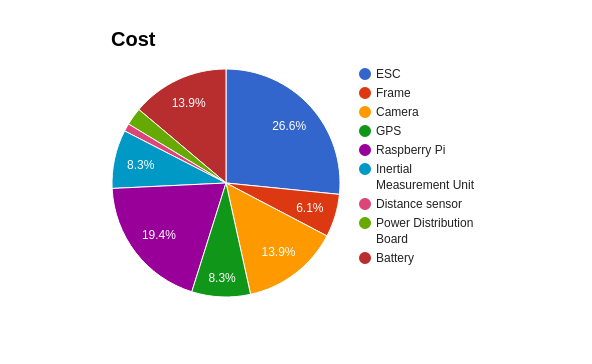
\includegraphics[width = 15cm]{cost.png}
  \caption{Project Cost for each Part}
  \label{Cost wise Estimate}	
\end{figure}

\begin{table}[H]
    \begin{tabular}{ | l | l | l | p{1cm}|}
    \hline
    S.No & Signal & Result \\ \hline
    1 & Swipe left joystick up & Quadcopter flies upward \\ \hline
    2 & Swipe left joystick down &  Quadcopter's height decreases \\ \hline
    3 & Swipe right joystick up & Quadcopter pitches forward \\ \hline
    4 & Swipe right joystick down & Quadcopter pitches backward \\ \hline
 5 & Swipe right joystick left & Quadcopter pitches left \\ \hline
 6 & Swipe right joystick right & Quadcopter pitches right \\ \hline
 7 & Click the 'start' camera button & Pi Camera starts shooting \\ \hline
 8 & Click the 'stop' camera button & Pi Camera stops shooting \\ \hline
 9 & Click the '+/-' button on the x-axis & Quadcopter's x-trim values change \\ \hline
 10 & Click the '+/-' button on the y-axis & Quadcopter's y-trim values change \\ \hline
\end{tabular}
\caption{Test Cases and Results}
\label{APT}
\end{table}

\subsection{Evaluation}
There are several changes that have to be made when flying the quadcopter in varying environments. The PID values change according to the wind conditions and other disturbances. Although the SD Card is securely inserted into the RPi, due to a large amount of vibration caused in the course of the quadcopter's flight, it may loosen leading to connection loss between the RPi and the App. 
\par
The quadcopter is controlled by the App from a distance of about 10-15 metres since communication occurs via WiFi. Images are taken by a RPi native camera which is fixed securely on top. The quality of the images taken largely depend on the stability of the quadcopter which are subject to the vagaries of the environment.
The pictures taken are stitched and/or reconstructed. The speed of the image-processing depends on the number of images taken and the quality of the images. 
\begin{figure}[H]
  \centering
  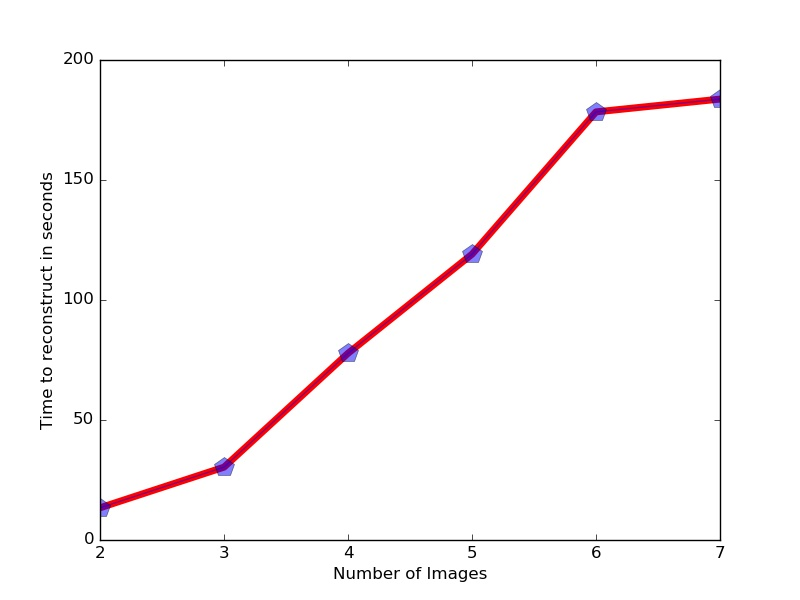
\includegraphics[width = 14cm]{pano.jpg}
  \caption{Time taken for computation of panorama stitching is directly proportional to the number of images. It stabilizes slightly when the image count is greater than seven.}
  \label{panorama stitching time graph} 
\end{figure}

Figures \ref{fig:filter}, \ref{fig:mop}, \ref{fig:pid} and \ref{fig:fpid} depict the data obtained during a test run of the quadcopter, where the sensor/output(y-axis) data is plotted against time in seconds(x-axis).
\par
The first 10 seconds show the data where the motors run at minimal speed, followed by intermittent high speeds to allow lift-off till the 20 second mark. At about 25 seconds the quadcopter had attained a height of roughly 1 feet from the ground and was hovering with mild oscillations. At about 45 seconds the quadcopter encountered a breeze causing it temporarily tilt in the direction of the breeze and oscillating with increasing amplitude till 55 seconds, at which point it was powered down.
\begin{figure}[H]
  \centering
  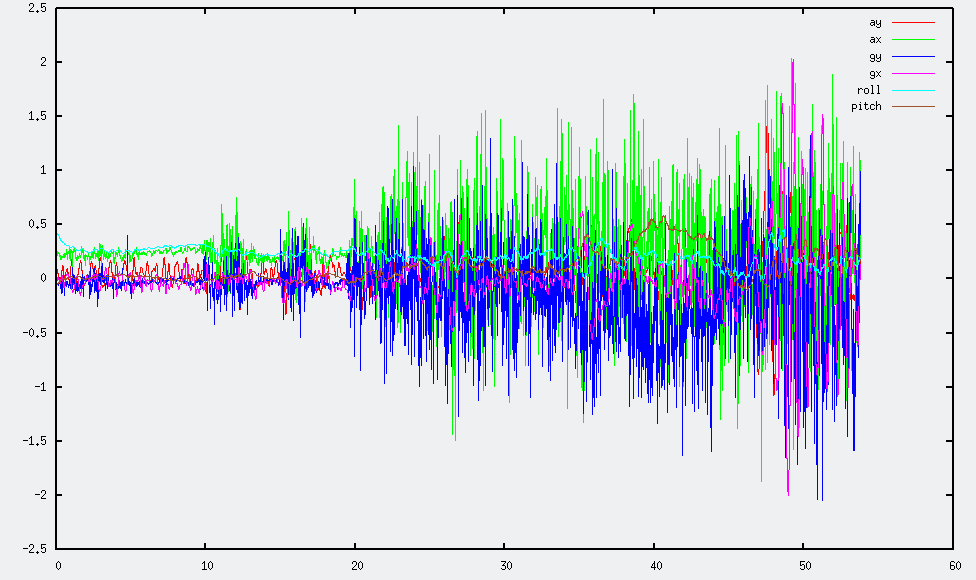
\includegraphics[width = 15cm]{complementary.png}
  \caption{Measurement of pitch and roll using complementary filter \label{fig:filter}}
  \label{Measurement of pitch and roll} 
\end{figure}
The orientation of the quadcopter is sensed using the accelerometer and the gyroscope present in the IMU sensor [Fig \ref{fig:filter}].
\par
An accelerometer measures all forces that are working on the object, it will also see a lot more than just the gravity vector. Every small force working on the object will disturb our measurement completely and result in noise[Fig \ref{fig:filter} ax and ay]. If we are working on an actuated system (like the quadrocopter), then the forces that drive the system will be visible on the sensor as well. The accelerometer data is reliable only on the long term, so a "low pass" filter has to be used.
\par
A Gyroscope measures accurately the change in angle[Fig \ref{fig:filter} gx and gy]. Accurate measurement of the current angle can be obtained that is not susceptible to external forces by integrating the change in angle over time to obtain the overall change in angle. However, due to the integration over time, the measurement has the tendency to drift, not returning to zero when the system goes back to its original position. The  data is reliable for a short term, since it drifts on the long term.
\par
The complementary filter combines the two the get a reliable sense of orientation[Fig \ref{fig:filter} pitch and roll]. On the short term, we use the data from the gyroscope, because it is very precise and not susceptible to external forces. On the long term, we use the data from the accelerometer, as it does not drift. The filter looks as follows:
\begin{equation}
angle = 0.98*(angle+gyrData*dt)+0.02*accData
\end{equation}
\par
The gyroscope data is integrated every timestep with the current angle value. After this it is combined with the low-pass data from the accelerometer (already processed with atan2). The constants (0.98 and 0.02) have to add up to 1 but can be changed to tune the filter properly.

\begin{figure}[H]
  \centering
  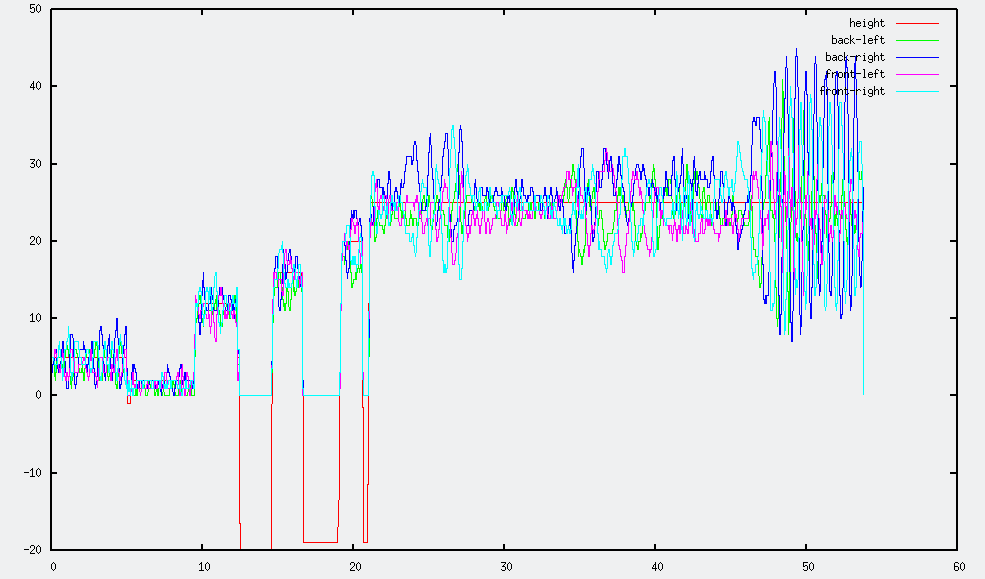
\includegraphics[width = 15cm]{motorsop.png}
  \caption{Output of motors with respect to height\label{fig:mop}}
  \label{Motor output}  
\end{figure}
The motor outputs require to be offset by the required height to allow the quadcopter to increase or decrease the overall height while balancing using the offset received from the PID controller[Fig \ref{fig:mop}].

\begin{figure}[H]
  \begin{subfigure}{1\textwidth}
    \centering
    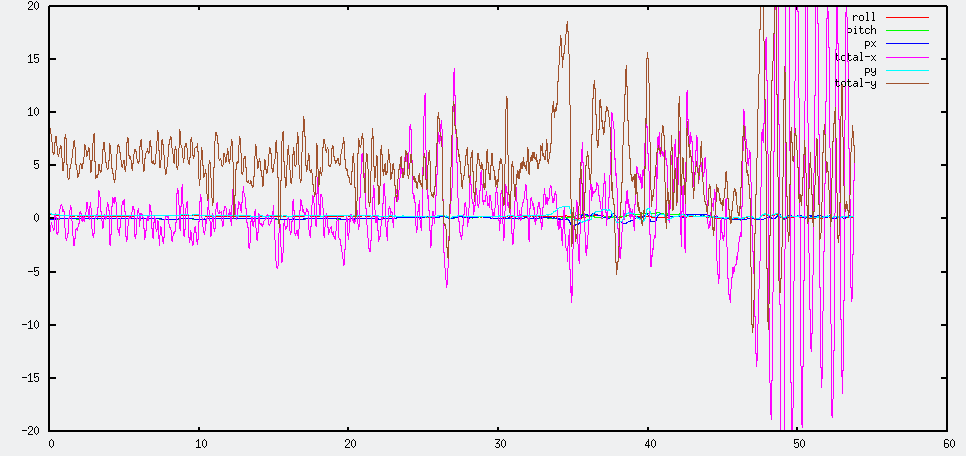
\includegraphics[width = 12cm]{pid.png}
    \caption{Derivation of output using PID controller\label{fig:pid}}
    \label{Motor output}  
  \end{subfigure}
  \begin{subfigure}{1\textwidth}
    \centering
    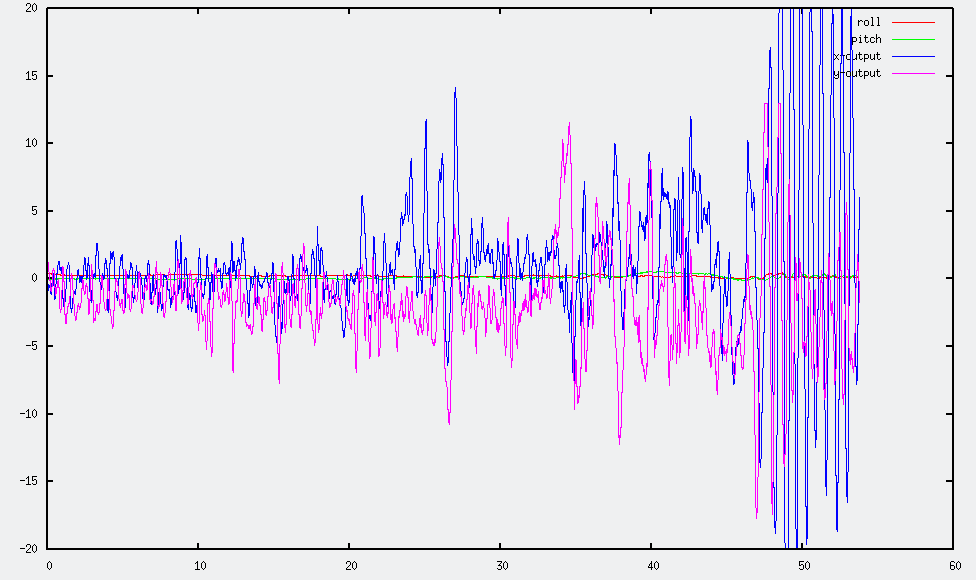
\includegraphics[width = 12cm]{output.png}
    \caption{Final output with respect to pitch and roll\label{fig:fpid}}
    \label{Measurement of pitch and roll} 
  \end{subfigure}
  \caption{Derivation and final output from sensed angles}
\end{figure}
Figure \ref{fig:pid} shows how the final output and Figure \ref{fig:fpid} shows how sensed pitch and roll are converted to the final output by the PID controller to be used as offset to the motor speed for balancing the quadcopter. The total-x and total-y are computed using the following PID formula:
\begin{equation}
motor_{command} = K_p^r*((K_p^a(\theta_{input} - \theta) + K_i^a\int (\theta_{input} - \theta)dt) -\frac{d\theta}{dt})
\end{equation}
\newline
The last chapter discusses the project's contributions and future work.
